Diante da visão da IoT propõe-se um estudo de caso no HNS (seção \ref{sec:hns}), com o intuito de verificar se é possível detectar efeitos colaterais indesejáveis. Para isto é idealizado um cenário, ``Levar Compras'' (seção \ref{sec:cenario}), dentro de um HNS (Figura \ref{fig:hnsworkmodel}). Neste, cada dispositivo da casa (veículo terrestre, elevador, garra mecânica) é disponibilizado como um serviço Web RESTFul. O HS do HNS é um servidor Web RESTFul com um FIM (seção\ref{sec:featureinteraction}) integrado, no qual será implantado um classificador para detecção de efeitos colaterais indesejáveis aplicavél ao cenário ``Levar Compras'', caso possa se construir um modelo com um grau de generalização aceitável (seção \ref{sec:constvalidacao}). A discussão do motivo de se utilizar dispositivos como serviços Web e, RESTFul em vez de SOAP foi realizada na seção \ref{subsec:dispositivosWeb}.

\begin{figure}[!htb] \centering 
  \centering
  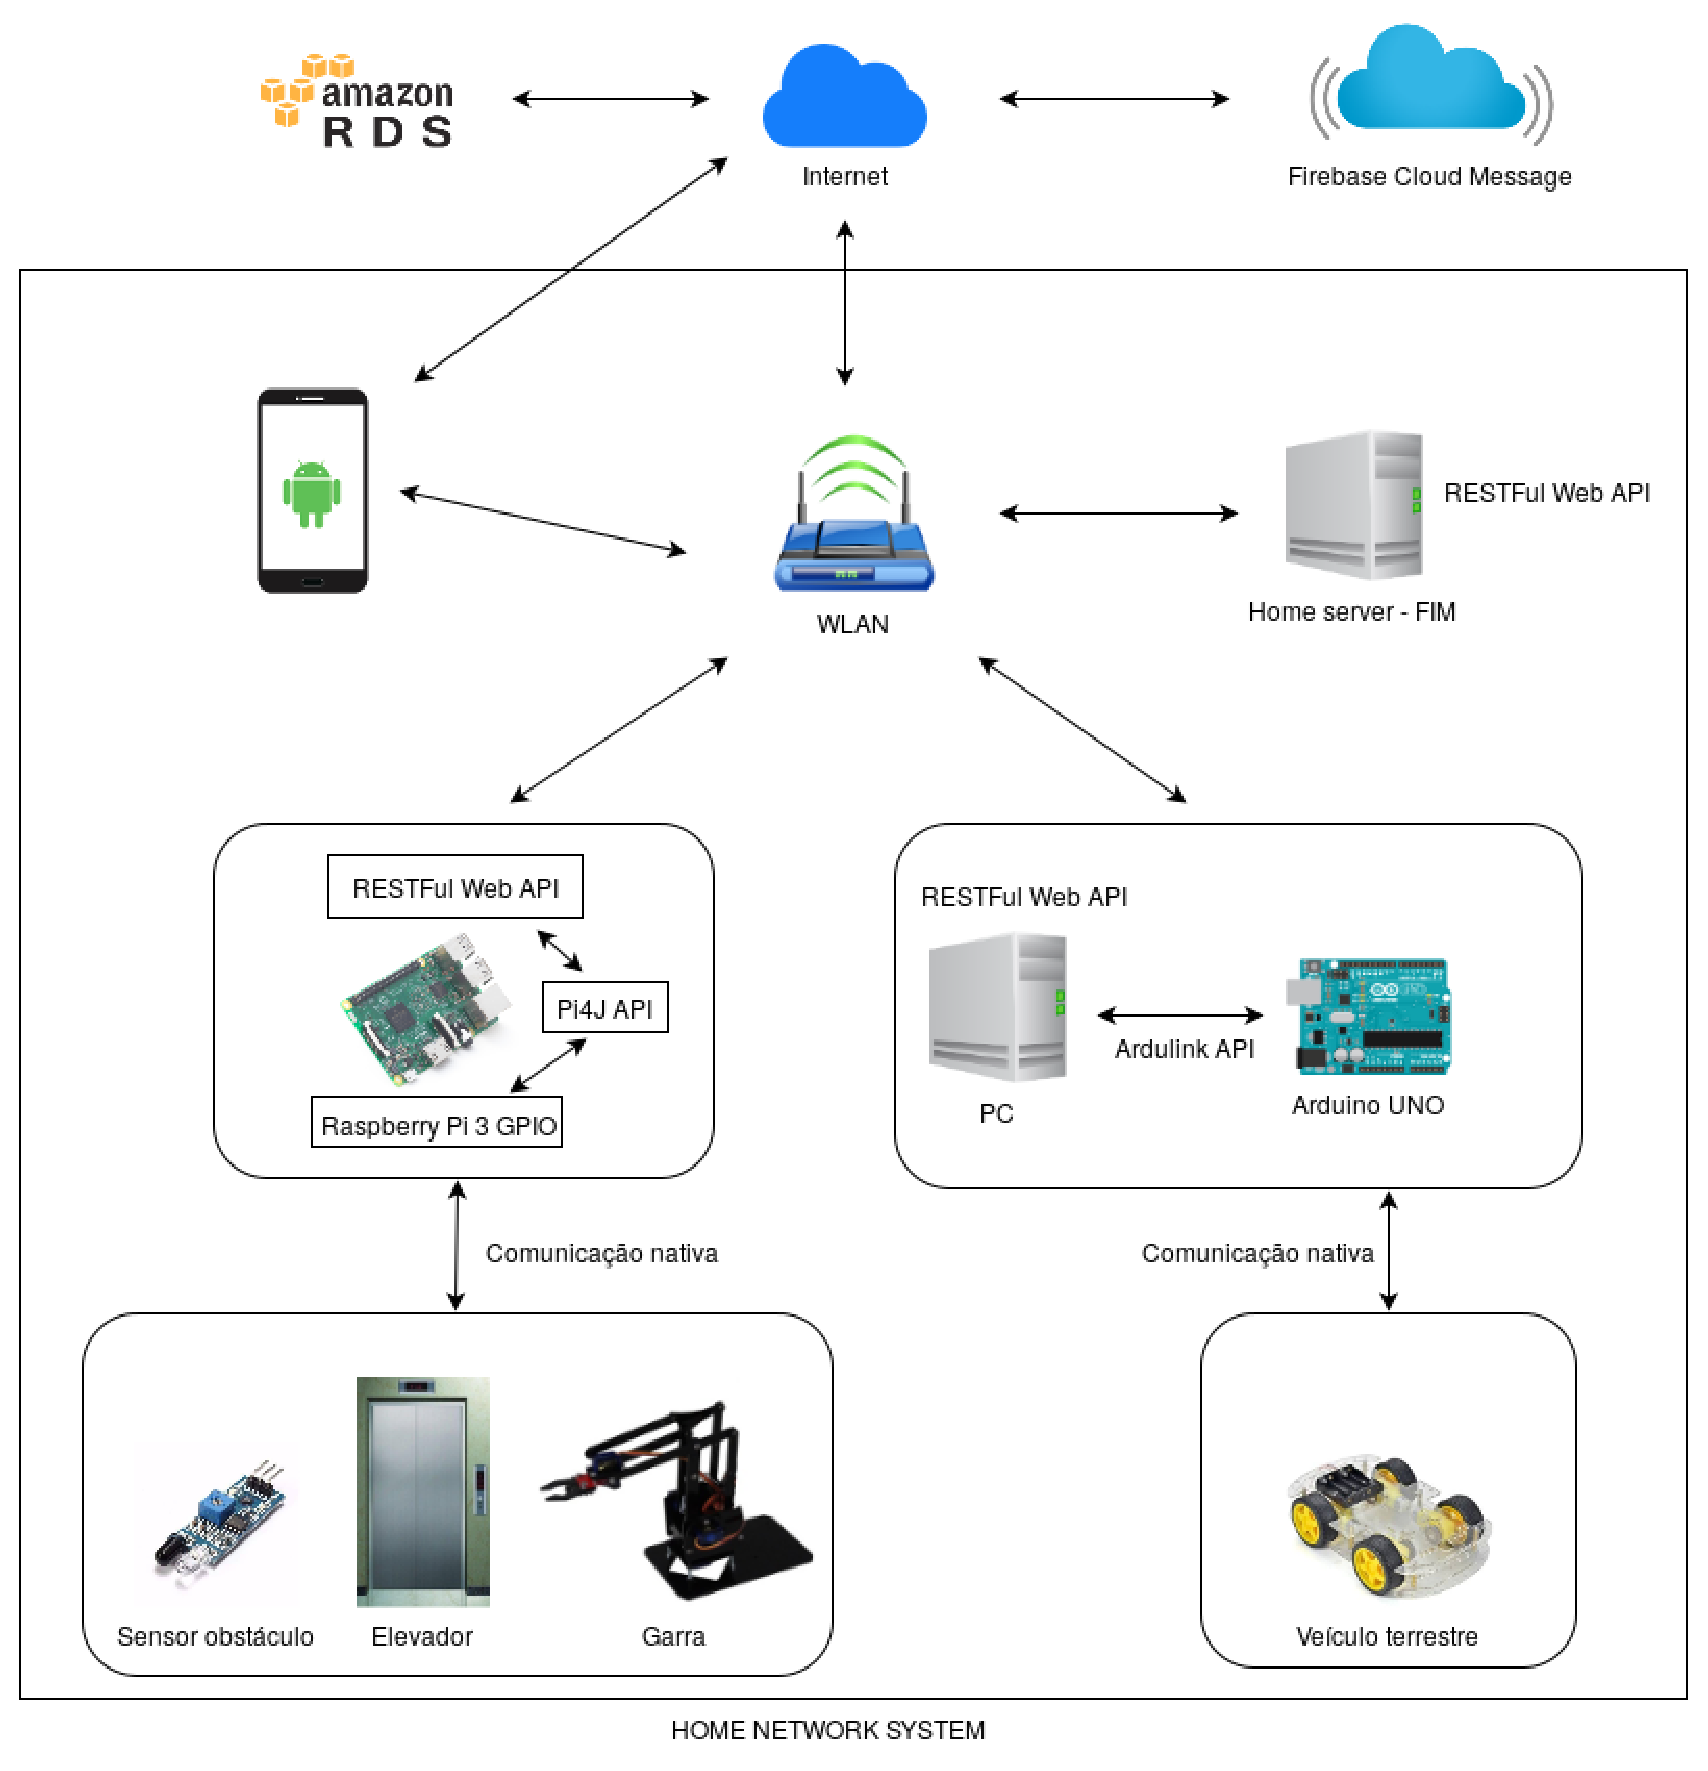
\includegraphics[width=1.0\columnwidth]{cenario} 
  \caption{Modelo do HNS utilizado neste trabalho.} 
  \label{fig:hnsworkmodel}
\end{figure}

\section{Cenário Levar compras}
\label{sec:cenario}
O cenário ``Levar compras'' refere-se a funcionalidade (\textit{feature} ou característica)  oferecida pelo HS. Esta característica é provida através da composição dos serviços do elevador, veículo e garra. O cenário em questão pode ser visualizado na Figura \ref{fig:cenario} e é descrito a seguir.

\begin{enumerate}
\item Um usuário da casa (morador ou visitante), organiza as compras numa cesta (que tem formato expansível) e a coloca sobre o veículo terrestre.
\item O usuário então aciona o serviço ``Levar compras'' (disponibilizado pelo HS) através do seu \textit{smartphone}. O serviço então começa sua execução.
\item O FIM solicita informações de restrições do elevador e veículo terrestre, assim como quais objetos compõem a cesta. Este então verifica se a cesta colocada sobre o carro quebrou alguma restrição do mesmo e se a massa total dos objetos excedem a carga máxima do elevador.
\item Se nenhuma destas restrições foram quebradas o FIM solicita ao veículo terrestre que leve a as compras até as proximidades do elevador.
\item Assim que o veículo chega no seu destino, este envia uma mensagem ao FIM informando de sua chegada.
\item O FIM então requisita o elevador para levar as compras.
\item O elevador agora solicita a garra mecânica que pegue o cesto e coloque-o dentro do elevador.
\item Quando a garra completa a execução do seu serviço, esta avisa ao elevador.
\item Caso não haja nenhuma restrição, como por exemplo, alguma coisa que possa impedir a porta do elevador de fechar, então o elevador inicia o transporte das compras ao seu destino final e manda uma notificação ao HS.
\item HS Captura token referente ao \textit{smartphone} com Android\footnotemark \footnotetext{\url{https://www.android.com/intl/pt-BR_br/}} do usuário da casa.
\item Por fim, o HS solicita ao serviço de notificação \textit{Firebase Cloud Message}\footnotemark \footnotetext{\url{https://firebase.google.com/docs/cloud-messaging/?hl=pt-br}} que envie uma notificação para o usuário da casa, que a recebe no seu \textit{smartphone}. Assim completa-se a execução do serviço ``Levar compras''.
\end{enumerate}
        
\begin{figure}[!htb] \centering 
  \centering
  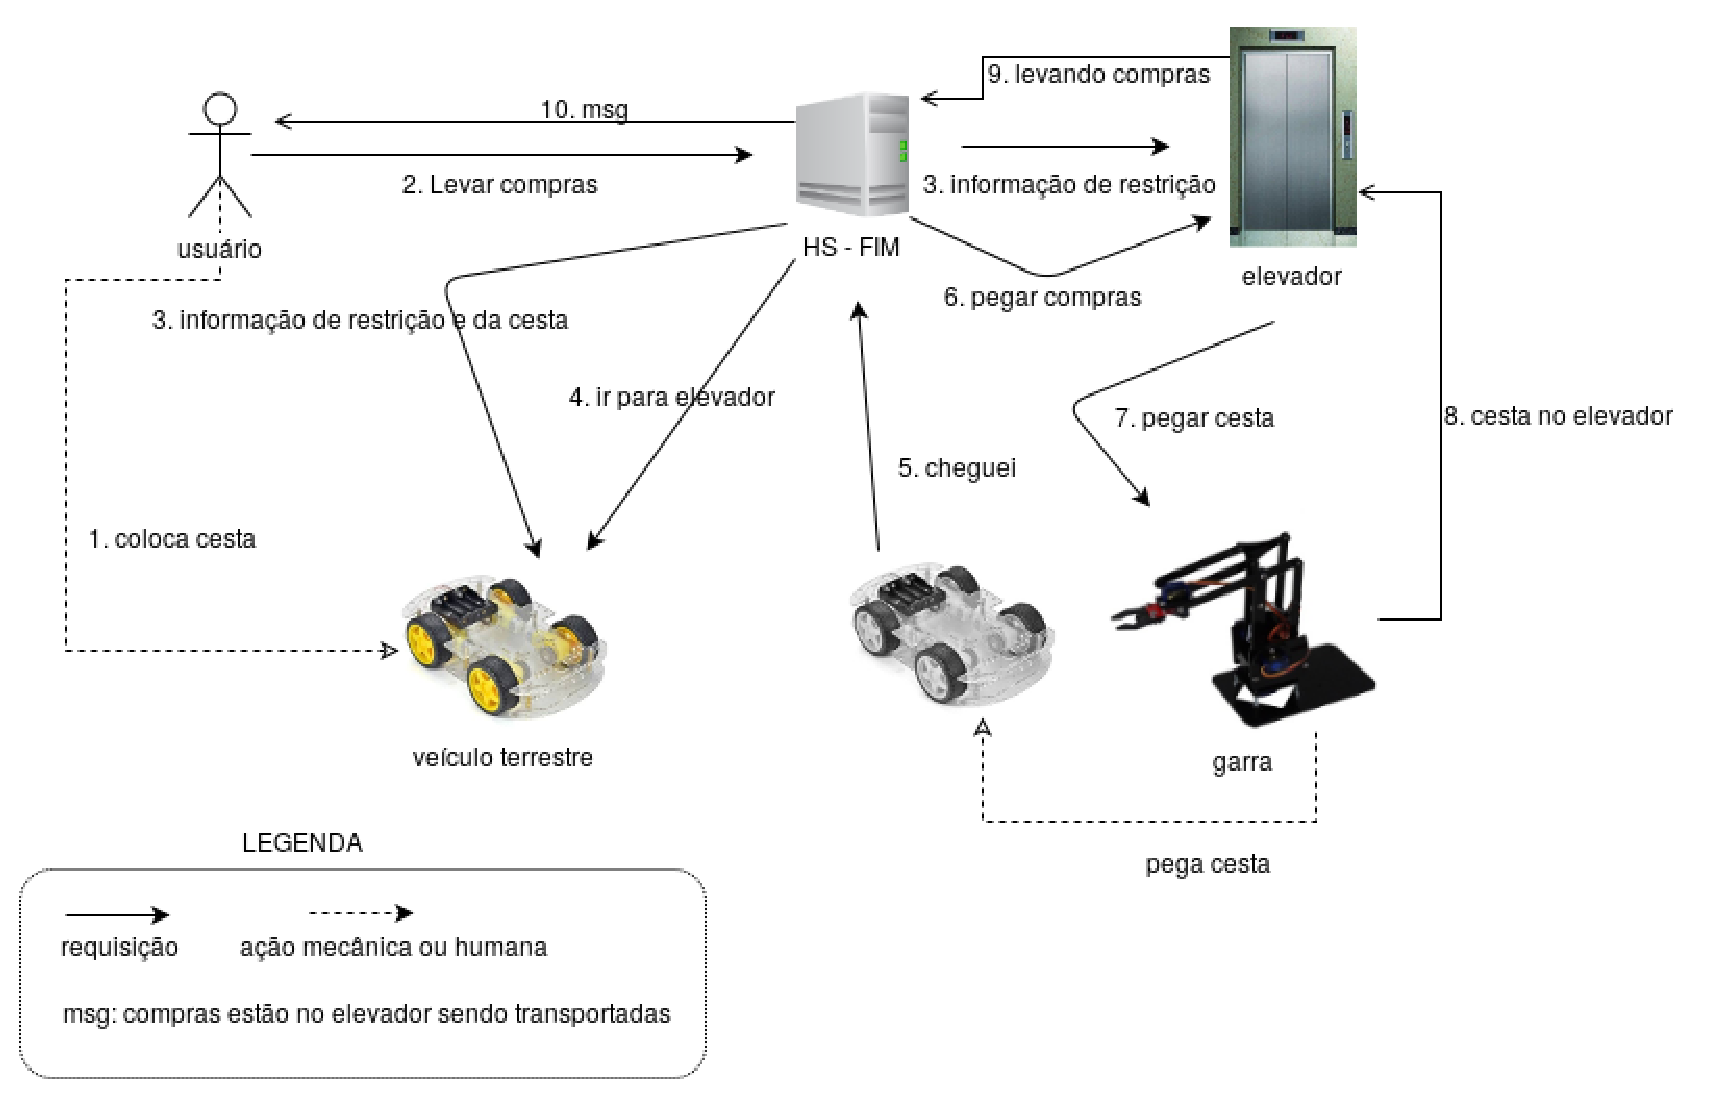
\includegraphics[width=1.0\columnwidth]{cenario_requests} 
  \caption{Cenário Levar compras.} 
  \label{fig:cenario}
\end{figure}

No cenário descrito da Figura \ref{fig:cenario} o elevador não contém motores nem algum outro tipo de sistema elétrico ou mecânico, este é representado por uma caixa de papelão e um sensor de obstáculo acoplado. O veículo terrestre é representado por um programa carregado no Arduino UNO\footnotemark \footnotetext{\url{https://www.arduino.cc/en/Main/ArduinoBoardUno}}, o qual escuta através de sua porta serial mensagens provindas do PC (Figura \ref{fig:cenario}) e as processa simulando as funcionalidades ``Ir para elevador'' e ``cheguei''. Pela mesma porta serial o veículo terrestre encaminha suas mensagens ao PC. Os dispositivos veículo, elevador e garra podem ser visualizados na Figura \ref{fig:cenario_real}.

\begin{figure}[!htb] \centering 
  \centering
  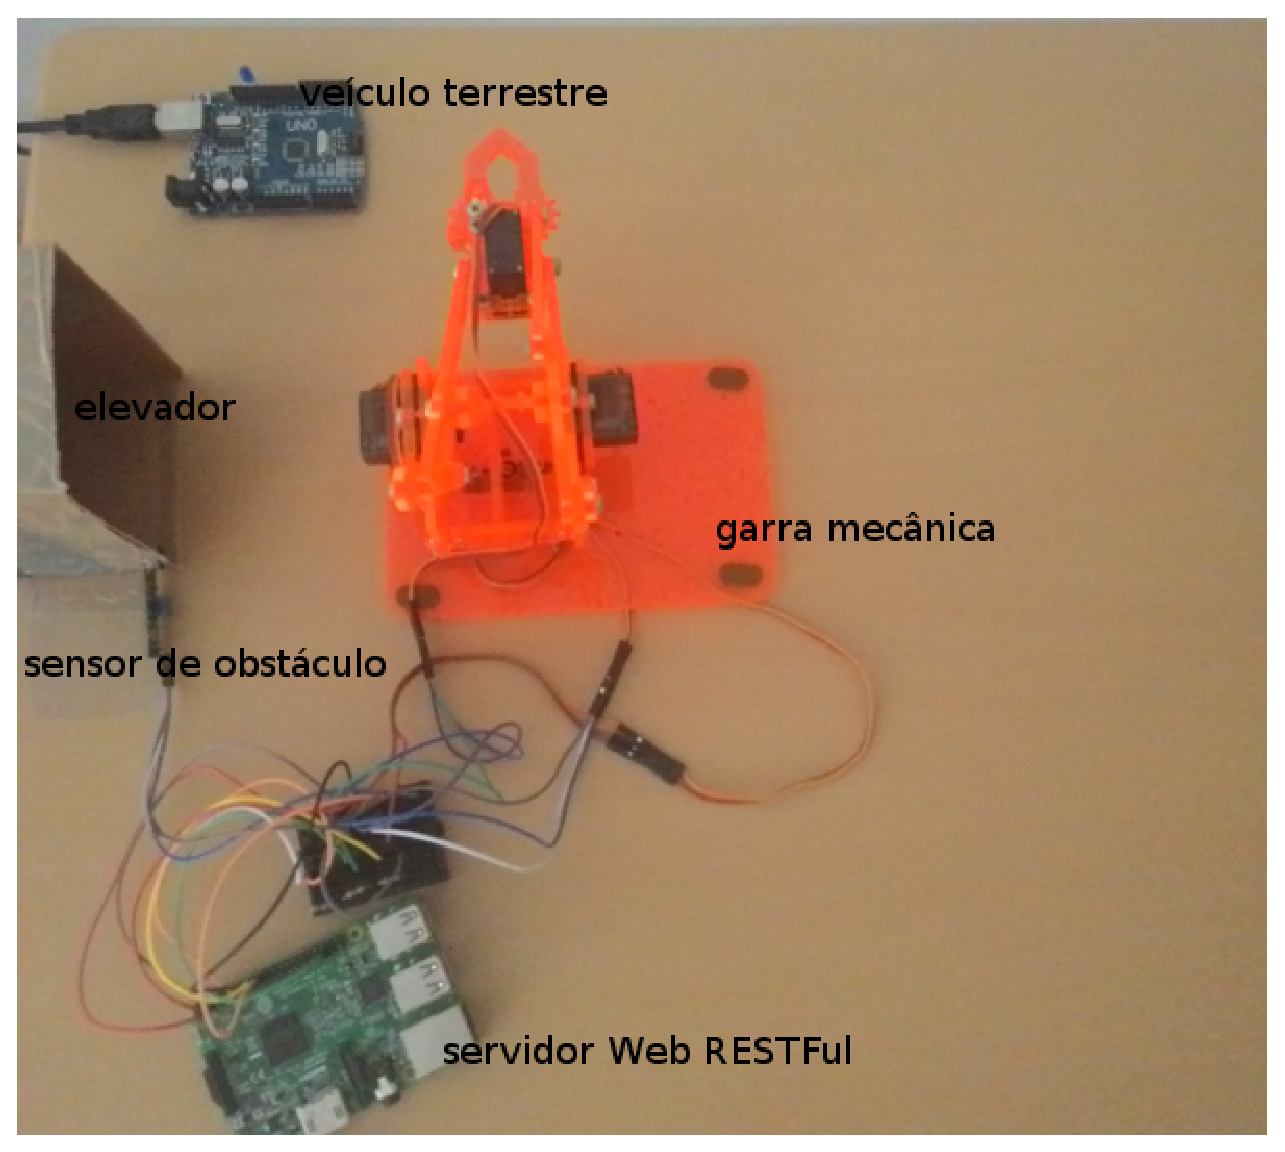
\includegraphics[width=0.8\columnwidth]{cenario_foto_real} 
  \caption{Dispositivos reais do cenário ``Levar compras''.} 
  \label{fig:cenario_real}
\end{figure}

\subsection{Execução do cenário Levar compras}
De acordo com a Figura \ref{fig:cenario} o primeiro passo para inicializar a execução do cenário é colocar a cesta no veículo terrestre. Apesar do veículo ser simulado através de um software embarcado no Arduino, este necessita das informações dos objetos que se deseja transportar. Sendo assim, as informações da cesta são passadas quando o usuário executa o passo 2 (Levar compras). O usuário digita o ``id da cesta'' (no banco de dados) que se deseja transportar e clica em um botão para inicializar o serviço. Todas as cestas são compostas com miniaturas de objetos que normalmente são encontrados em supermercados, exemplos de cestas podem ser visualizados na Figura \ref{fig:exemplos_cesta}. Todos os objetos e cestas estão cadastradas no banco de dados na nuvem (amazon RDS\footnotemark \footnotetext{\url{https://aws.amazon.com/pt/rds/postgresql/}}), o qual foi apresentado na Figura \ref{fig:hnsworkmodel}. A lista de objetos que podem fazer parte de uma cesta é demonstrada na Figura \ref{fig:lista_objetos}, observe que para cada objeto é cadastrado suas características de massa, largura, comprimento, altura e diâmetro.

\begin{figure}[!htb] \centering 
  \centering
  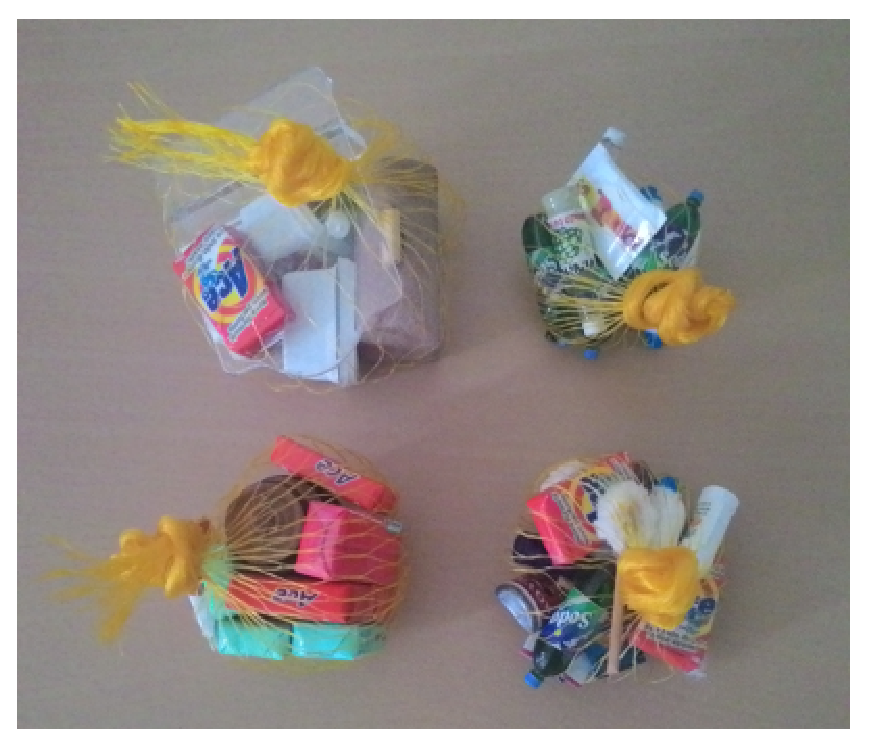
\includegraphics[width=0.8\columnwidth]{experimento/exemplos_cesta} 
  \caption{Exemplo de cestas do cenário ``Levar compras``.} 
  \label{fig:exemplos_cesta}
\end{figure}

\begin{figure}[!htb] \centering 
  \centering
  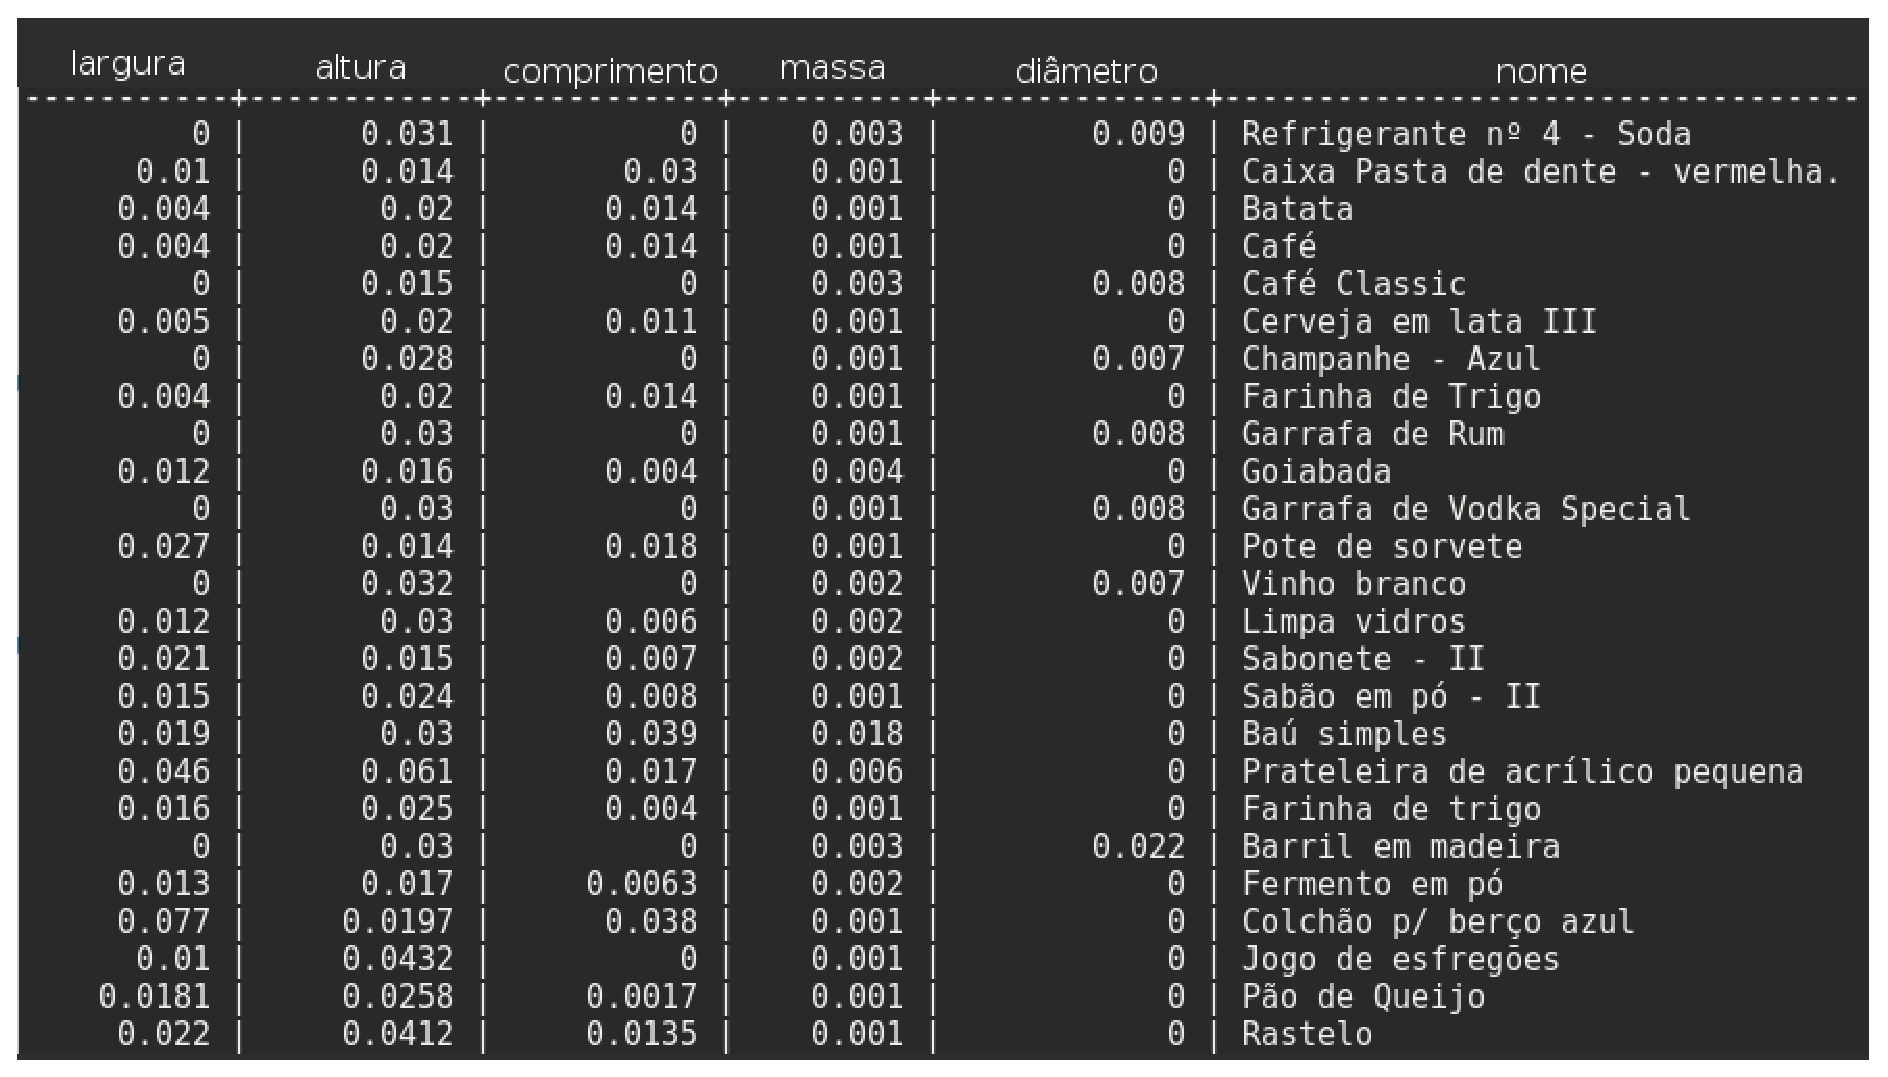
\includegraphics[width=0.8\columnwidth]{experimento/lista_items} 
  \caption{Lista dos objetos que podem ser utilizados para compor uma cesta.} 
  \label{fig:lista_objetos}
\end{figure}

Os próximos passos (3, 4, 5, e 6) do cenário podem ser executados sem mais problemas, pois já têm toda a informação necessária e não necessita de nenhuma intervenção humana. Isto já não acontece com o passo 7 (pegar cesta), pois este necessita de intervenção humana para a garra poder pegar a cesta e continuar a realizar o seu serviço, é preciso posicionar a cesta no lugar correto para a garra prender a cesta, como pode ser visto na Figura \ref{fig:garra_pegando_objeto}. Então, após a garra executar seu serviço esta manda uma mensagem para o elevador e, caso não tenha nada obstruindo a porta do elevador este inicia o transporte da cesta até o local desejado e manda uma mensagem para o FIM. Daí em diante a execução do cenário continua da mesma forma com já explanado.

\begin{figure}[!htb] \centering 
  \centering
  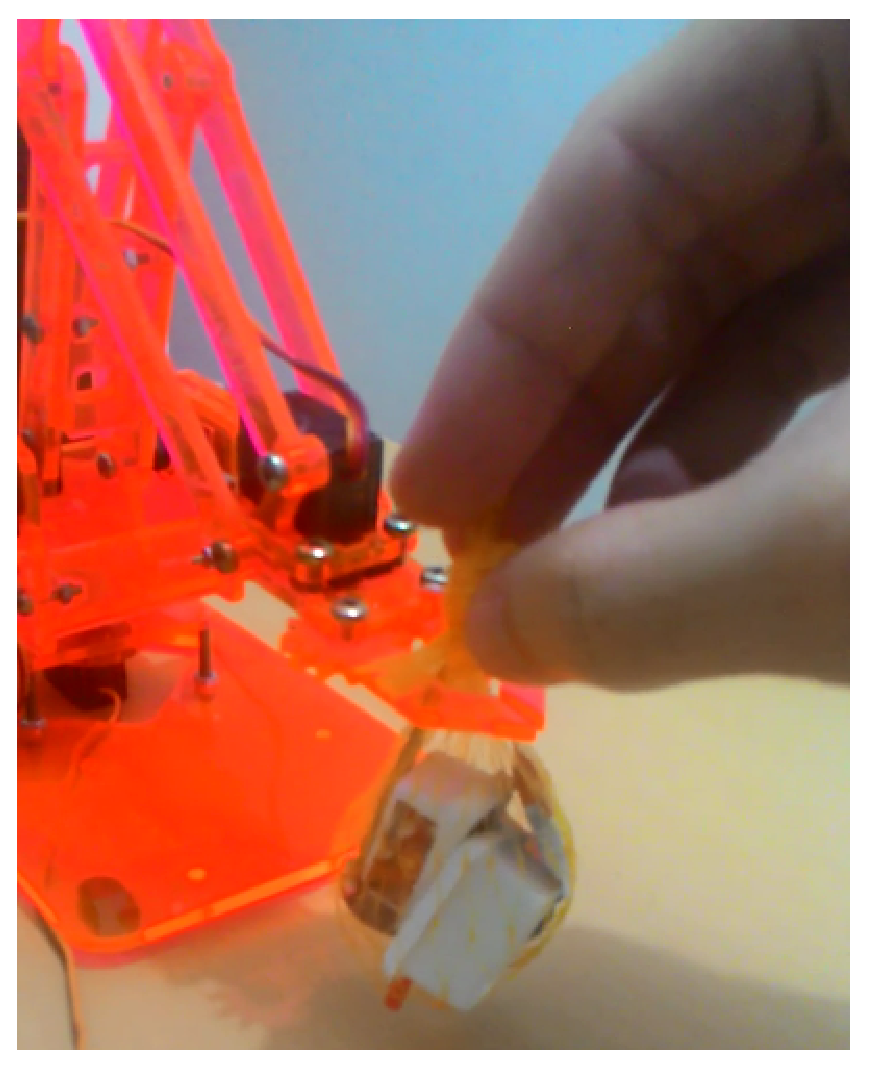
\includegraphics[width=0.8\columnwidth]{experimento/garra_pegando_objeto} 
  \caption{Cesta posicionada no local adequado por um humano, para que a garra possa prender a cesta adequadamente.} 
  \label{fig:garra_pegando_objeto}
\end{figure}

\subsection{Observação do problema}
\label{subsec:obsproblema}
Para a execução deste cenário foram confeccionadas e cadastradas no banco 59 cestas distintas. Antes de registrar as cestas no banco sempre era observado se a cesta cabia dentro do elevador quando colocadas de forma manual, e se também não ultrapassava os limites da porta, o limite de detecção do sensor de obstáculos. Então a cesta só era registrada caso coubesse no elevador e não estivesse em área que pudesse obstruir a porta.

O cenário foi executado 59 vezes, uma para cada cesta, e pode-se observar que em algumas vezes o comportamento da garra provocava um efeito colateral indesejável (seção \ref{sec:featureinteraction}) na funcionalidade ``Levar compras'', pois a garra durante a execução do seu serviço (pegar cesta, mover de uma lado a outro , largar cesta) acabava por vezes não conseguindo que a cesta ficasse disposta dentro do elevador de uma maneira em que este pudesse continuar com o serviço de ``Levar compras'', mesmo que para todos esses casos se esperasse sempre como resultado o elevador levar as compras sem problemas, já que se era sabido que as cestas cabiam no elevador e, nenhuma delas feria as restrições de massa do carro nem do elevador. Tanto o veículo quanto o elevador sempre funcionaram de maneira esperada nestas execuções, pois o veículo sempre levava a carga para o local destinado avisando quando chegasse, e o elevador sempre acionava o serviço da garra, levava a carga  e avisava ao FIM quando não tinha obstáculo na porta, enquanto deixava de levar quando tinha, funcionando de maneira correta quanto as especificações de sua funcionalidade de locomoção, mas indo contra o comportamento esperado da funcionalidade pai ``Levar carga''. 

Concluindo as observações feitas até agora, o comportamento da garra junto com os tipos de objetos presentes na cesta faziam com que algumas vezes ocorressem locomoção destes durante o transporte da garra, e também no momento em que os objetos eram postos no compartimento do elevador. Nesse momento, os objetos as vezes geravam outras dimensões de cesta e/ou deslocamento da mesma, devido a natureza dos objetos e da forma como os objetos eram soltos pela garra. Sendo assim, para tentar detectar esses efeitos colaterais indesejáveis através do DECORATE, utilizou-se dos valores das grandezas físicas dos objetos (altura, massa, largura, comprimento, diâmetro) para gerar características que pudessem ser interessantes para a construção de modelos de classificadores satisfatórios (seção \ref{sec:constvalidacao}). Vale salientar que esta informação da cesta é uma resposta do veículo terrestre referente a requisição ``3'' da Figura \ref{fig:cenario}, ou seja, é uma das informações que os dispositivos e/ou serviços trocam entre si durante a excecução de algum serviço.

Como todas as cestas estavam previamente cadastradas no banco de dados, a estas foram atribuídos valores de ``é efeito colateral'' ou ``não é efeito colateral'', a medida que se observava cada execução do cenário. Desta forma, será considerado para detecção de efeitos colaterais indesejáveis as informações das cestas.

\section{Seleção dos dados}
\label{sec:selecaodados}
Os dados coletados na etapa de execução do cenário ``Levar carga'', 59 cestas, ainda estão muito brutos, observe que uma cesta deve conter pelo menos um objeto, como também pode conter muitos. Supomos que a cesta tenha 10 objetos, então o total de características da cesta seria $10.5=50$, pois cada objeto possui cinco características. Utilizar as características dos objetos desta forma, além de provavelmente não predizer nada em um modelo de classificação, terá um custo computacional muito elevado. Para diminuir a quantidade de atributos e melhor qualificá-los gerou-se características a partir de todos os atributos dos objetos da cesta: média das alturas, dos comprimentos, das larguras, dos diâmetros e das massas, assim como o total de cada uma dessas medidas, e o total de itens. De ínicio então têm-se a seleção de 11 parâmetros.

Com a seleção prévia desses atributos, constriu-se um arquivo ``arff'', que é o tipo de arquivo padrão utilizado como \textit{dataset} pelo Weka \cite{Hall:2009}. Este \textit{dataset} é composto de 59 instâncias (referente as 59 cestas), cada uma com 11 atributos mais um que identifica a qual classe pertence. Então têm-se 11 atributos númericos e um nominal (a classe a qual a instância pertence).

O próximo passo utilizado nesse processo de seleção de atributos foi o de visualizar estes novos parâmetros par a par, e verificar quais pares parecem melhor separar as classes ``é efeito colateral'' ou ``não é efeito colateral''. A Figura \ref{fig:plotall1} passa a ideia de tal visualização. Dentre essas plotagens foram selecionadas três da Figura \ref{fig:eixos_4_atributos}, as quais aparentam melhor separar as classes, são respectivamente os pares ordenados (somaLargura, somaMassa) - ``sl x sm'', (somaDiâmetro, somaLargura) - ``sd x sl'' e, (médiaAltura, somaLargura) - ``ma x sl''. Então, nesta fase de seleção dos atributos, estes foram os pares selecionados para construção e validação do modelo (seção \ref{sec:constvalidacao} seguinte). Observe que o espaço de \textit{features} foi reduzido a duas características.

\begin{figure}[!htb] \centering 
  \centering
  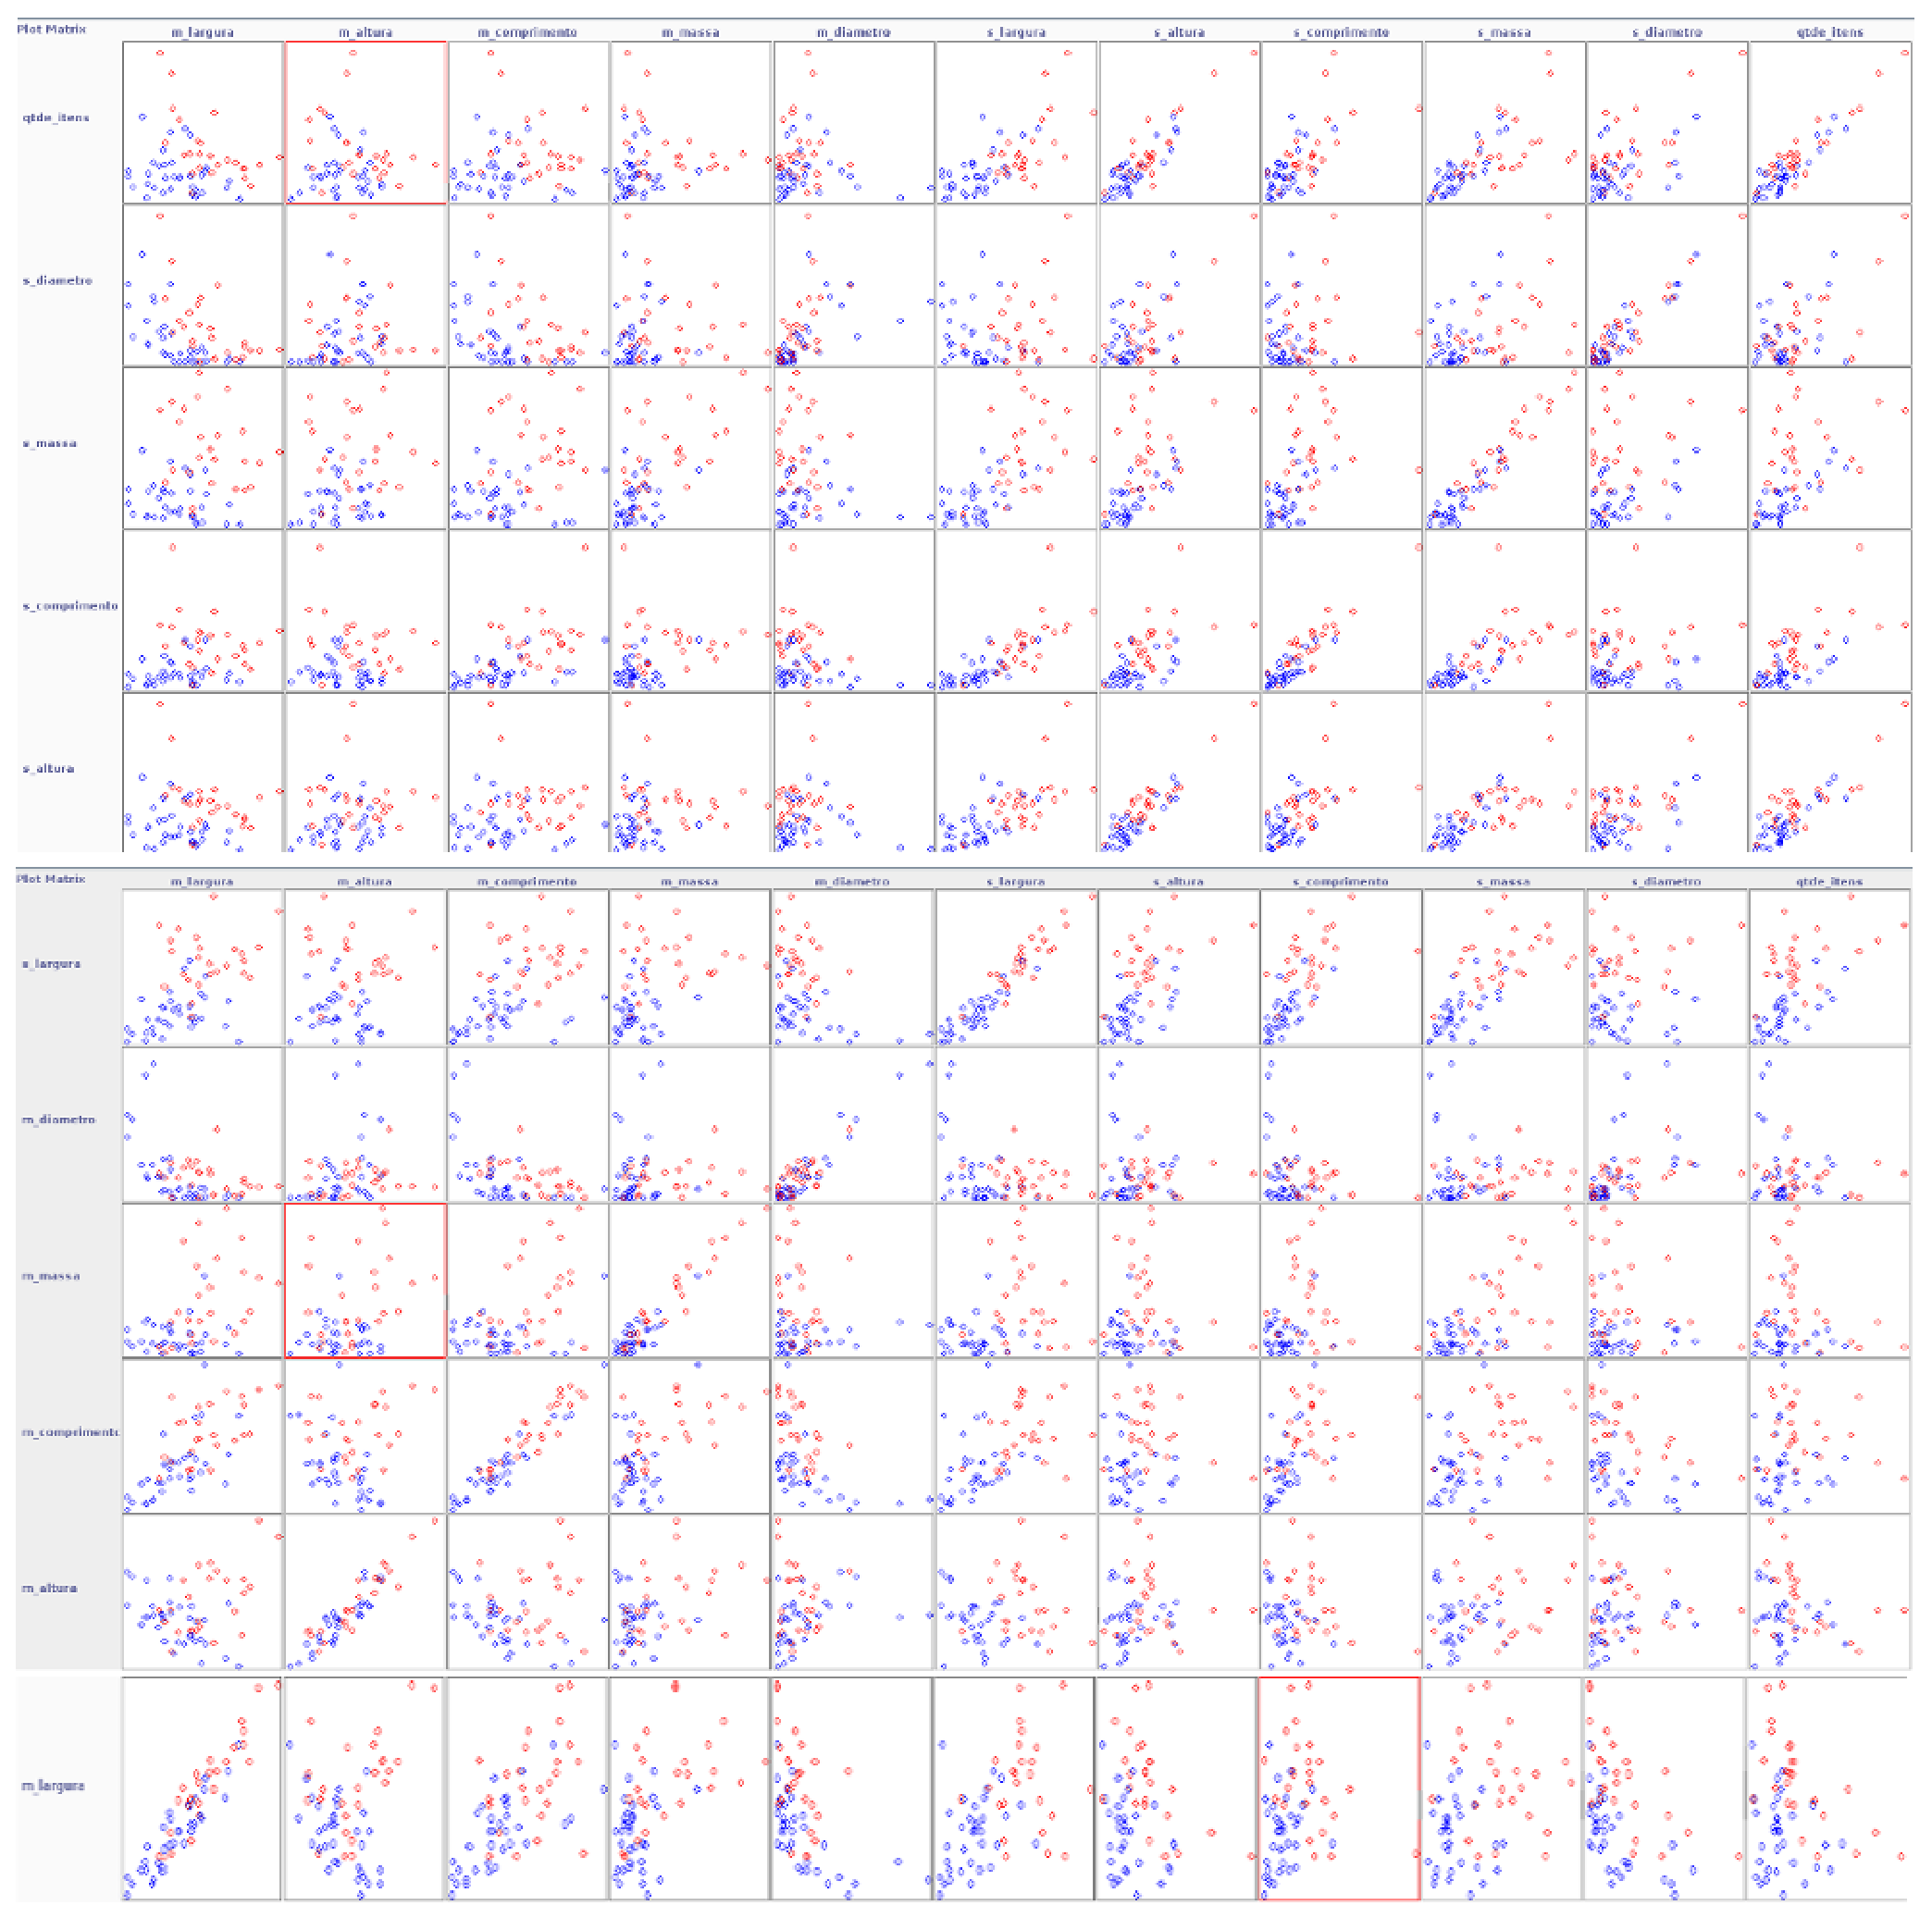
\includegraphics[width=1.0\columnwidth]{experimento/all_plot} 
  \caption{Plotagem do espaço de \textit{features} par a par do \texit{dataset} de 59 instâncias.} 
  \label{fig:plotall1}
\end{figure}

\begin{figure}[!htb] \centering 
  \centering
  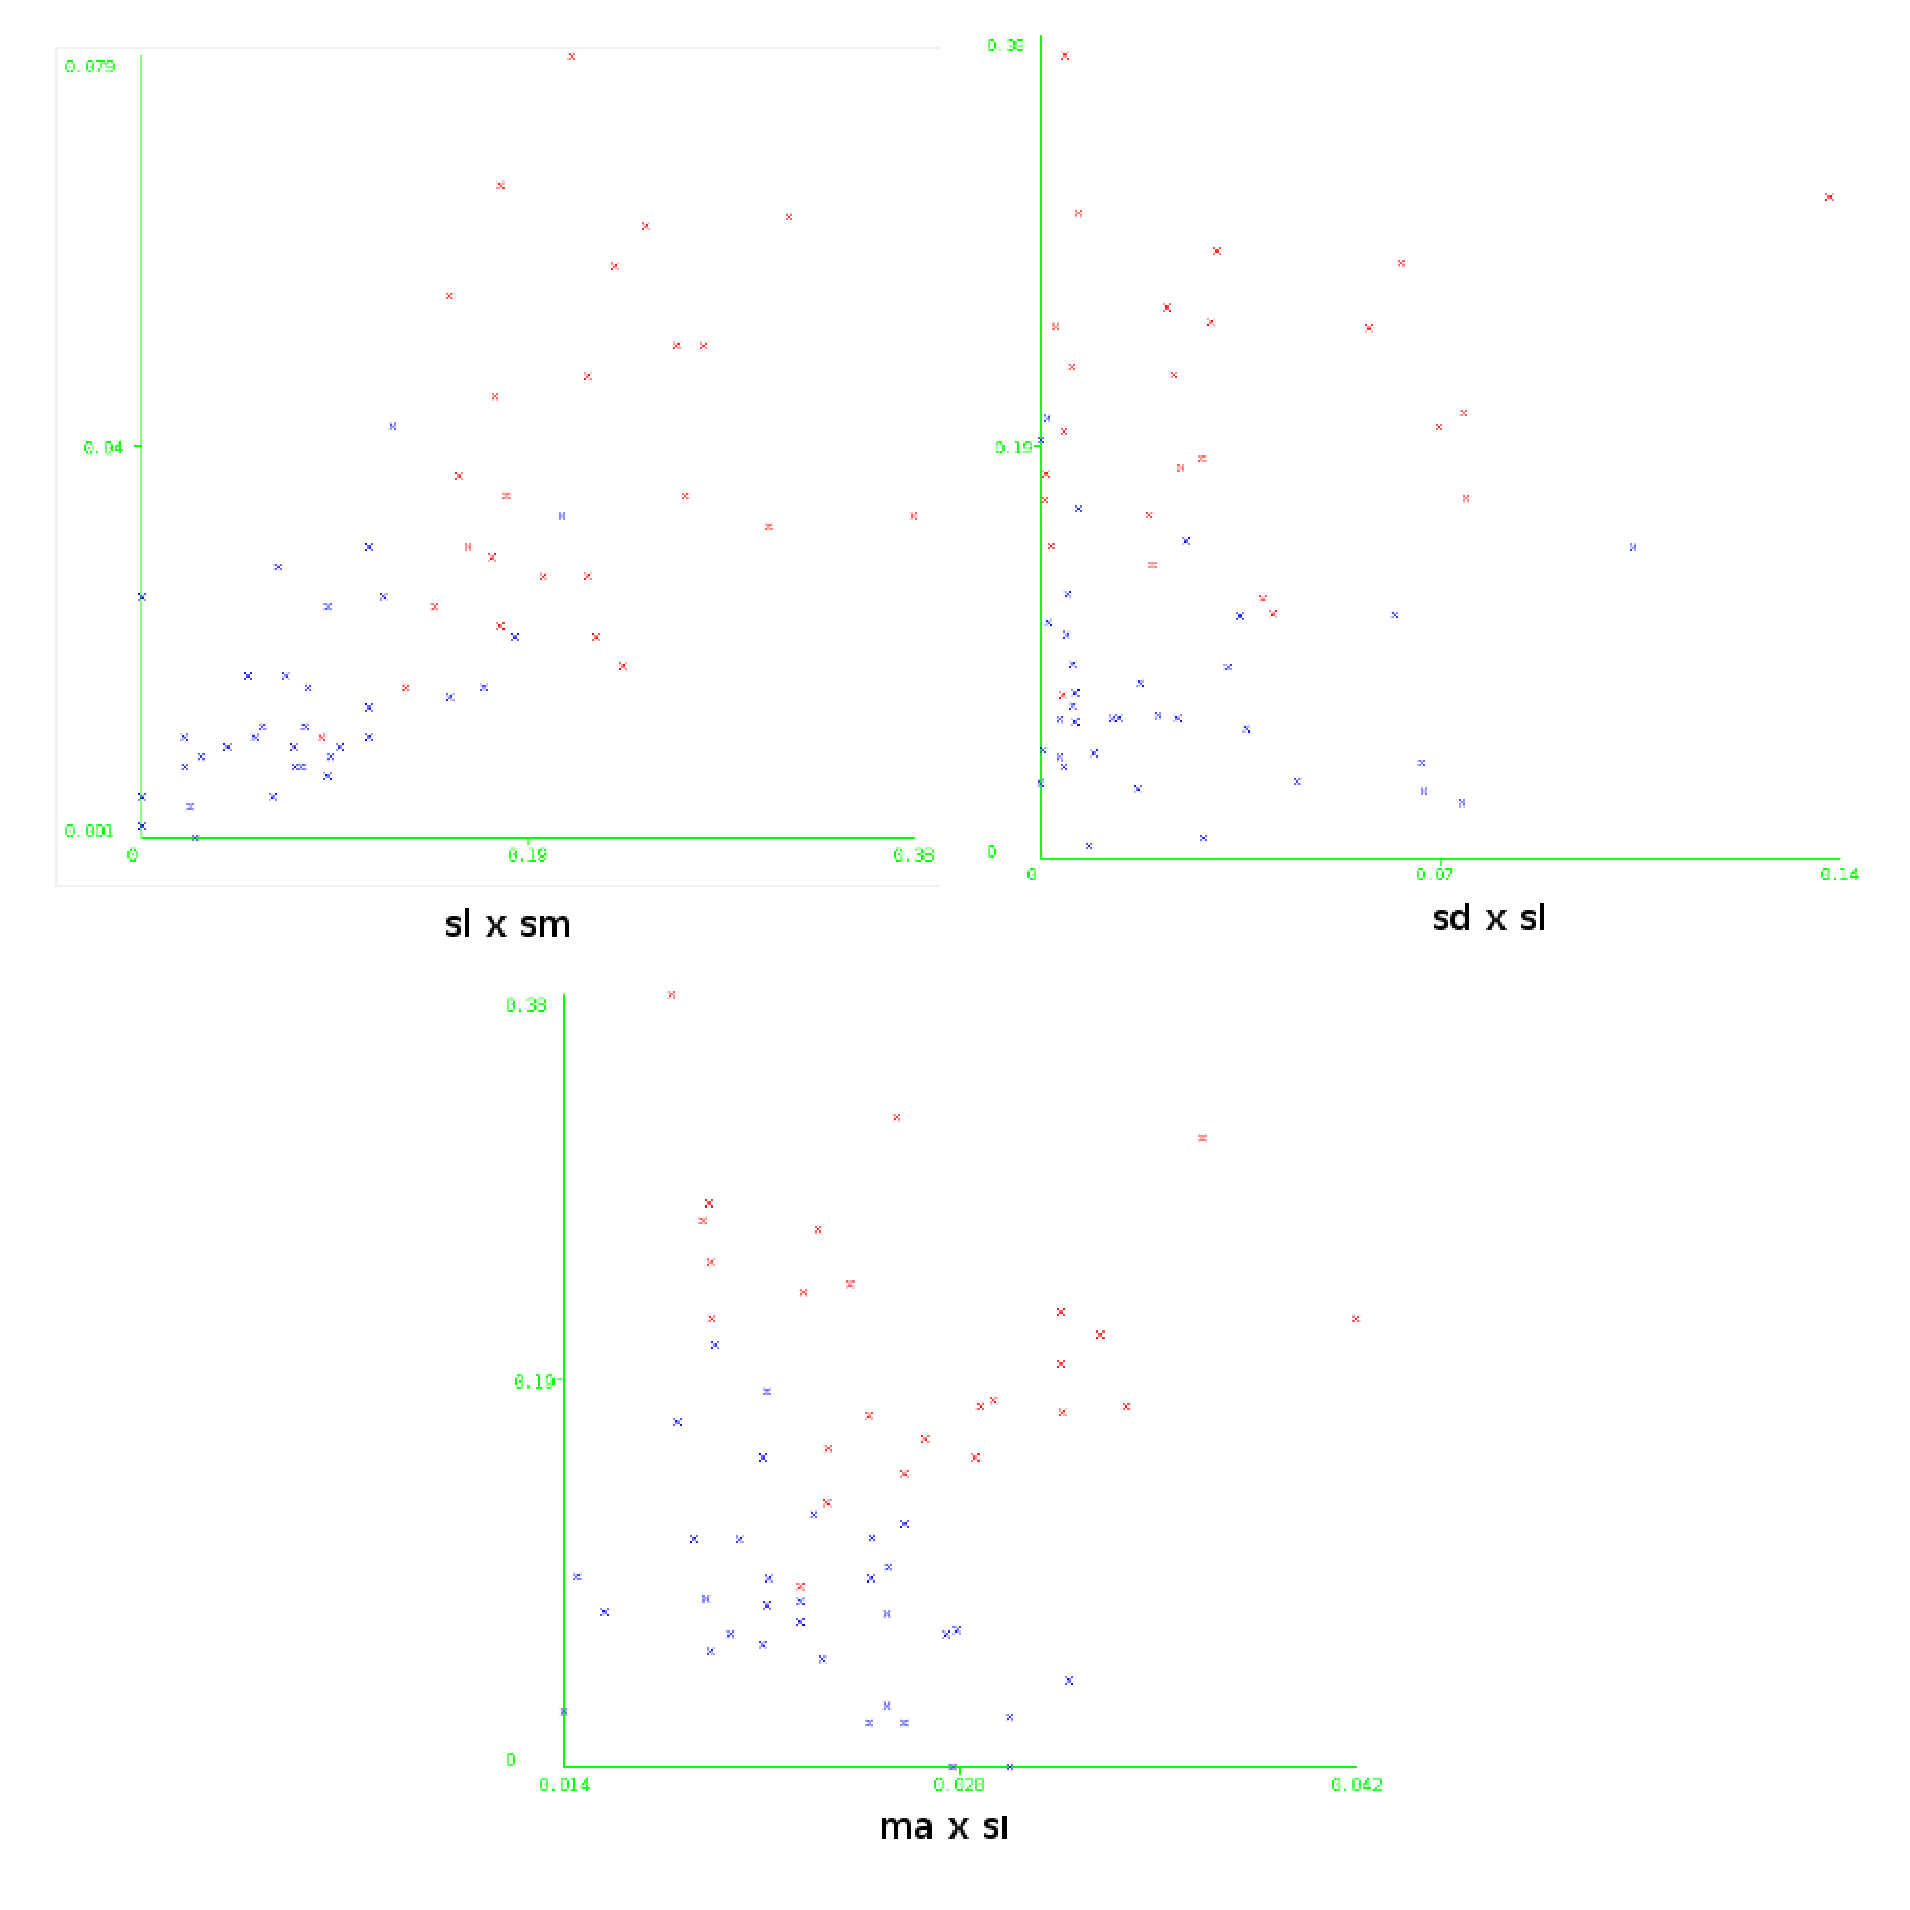
\includegraphics[width=0.8\columnwidth]{experimento/eixos_4_atributos} 
  \caption{Separação das classes entre os atributos (somaLargura, somaMassa) - ``sl x sm'', (somaDiâmetro, somaLargura) - ``sd x sl'' e, (médiaAltura, somaLargura).} 
  \label{fig:eixos_4_atributos}
\end{figure}

\section{Validação do modelo de classificador}
\label{sec:constvalidacao}
Diante dos pares de atributos selecionados na etapa anterior (seção \ref{sec:selecaodados}), utilizou-se o método \textit{stratified-10-fold-cross-validation} (repetido dez vezes) juntamente com o \textit{ensemble DECORATE} a fim de se construir e verificar se é possível generalizar pelo menos um modelo. 

Em cada validação construi-se um modelo com diferentes frações do dataset, variando de 16 instâncias a 59 instâncias. Os parâmetros do DECORATE escolhidos neste trabalho foram semelhantes a um dos testes avaliativos realizados em \cite{Melville:2004}, nos quais comparam \textit{DECORATE} com outros métodos classificatórios, em diferentes tamanhos de dataset e diferentes parâmetros do DECORATE. Para as avaliações neste trabalho o número de iterações é setado em 50, o número máximo de classificadores participantes no \textit{ensemble} é setado em 14, o classificador base utilizado é o J48 e, a quantidade de exemplos artificiais gerados em cada iteração é setado para 100\% (valores setados de 50\% a 100\% não faz variar muito o resultado \cite{Melville:2004}) do tamanho do dataset de treino. Os resultados das avaliações podem ser vistos na Figura \ref{fig:accuracy_precision_recall}. Nesta percebe-se um domínio quase absoluto da curva pontuada de aprendizado verde (médiaAltura, somaLargura - ``ma x sl''). Por esso motivo essa será a curva analisada para escolher um modelo o mais adequado possível para implantar no FIM. Como o principal motivo da implantação do classificador no FIM é detectar efeitos colaterais indesejáveis, então pretende-se que o modelo tenha um alto índice de \textit{recall}, pois não se deseja que se tenha muitos falso negativos, ou seja, muitos casos classificados como não sendo efeito colateral, mas que na verdade era. Visualizando a curva percebe-se que esta têm um crescimento acentuado e depois torna-se estável a partir do dataset com 30 instâncias. Logo fará-se uma análise a partir deste ponto. Os maiores valores de \textit{recall} partindo deste ponto são aqueles quando o \textit{dataset} tem 40 ou mais instâncias, para todos estes pontos considera que se obteve um bom grau de generalização. Estes valores podem ser visualizados na Tabela \ref{table:valorescurva}. 

\begin{figure}[!htb] \centering 
  \centering
  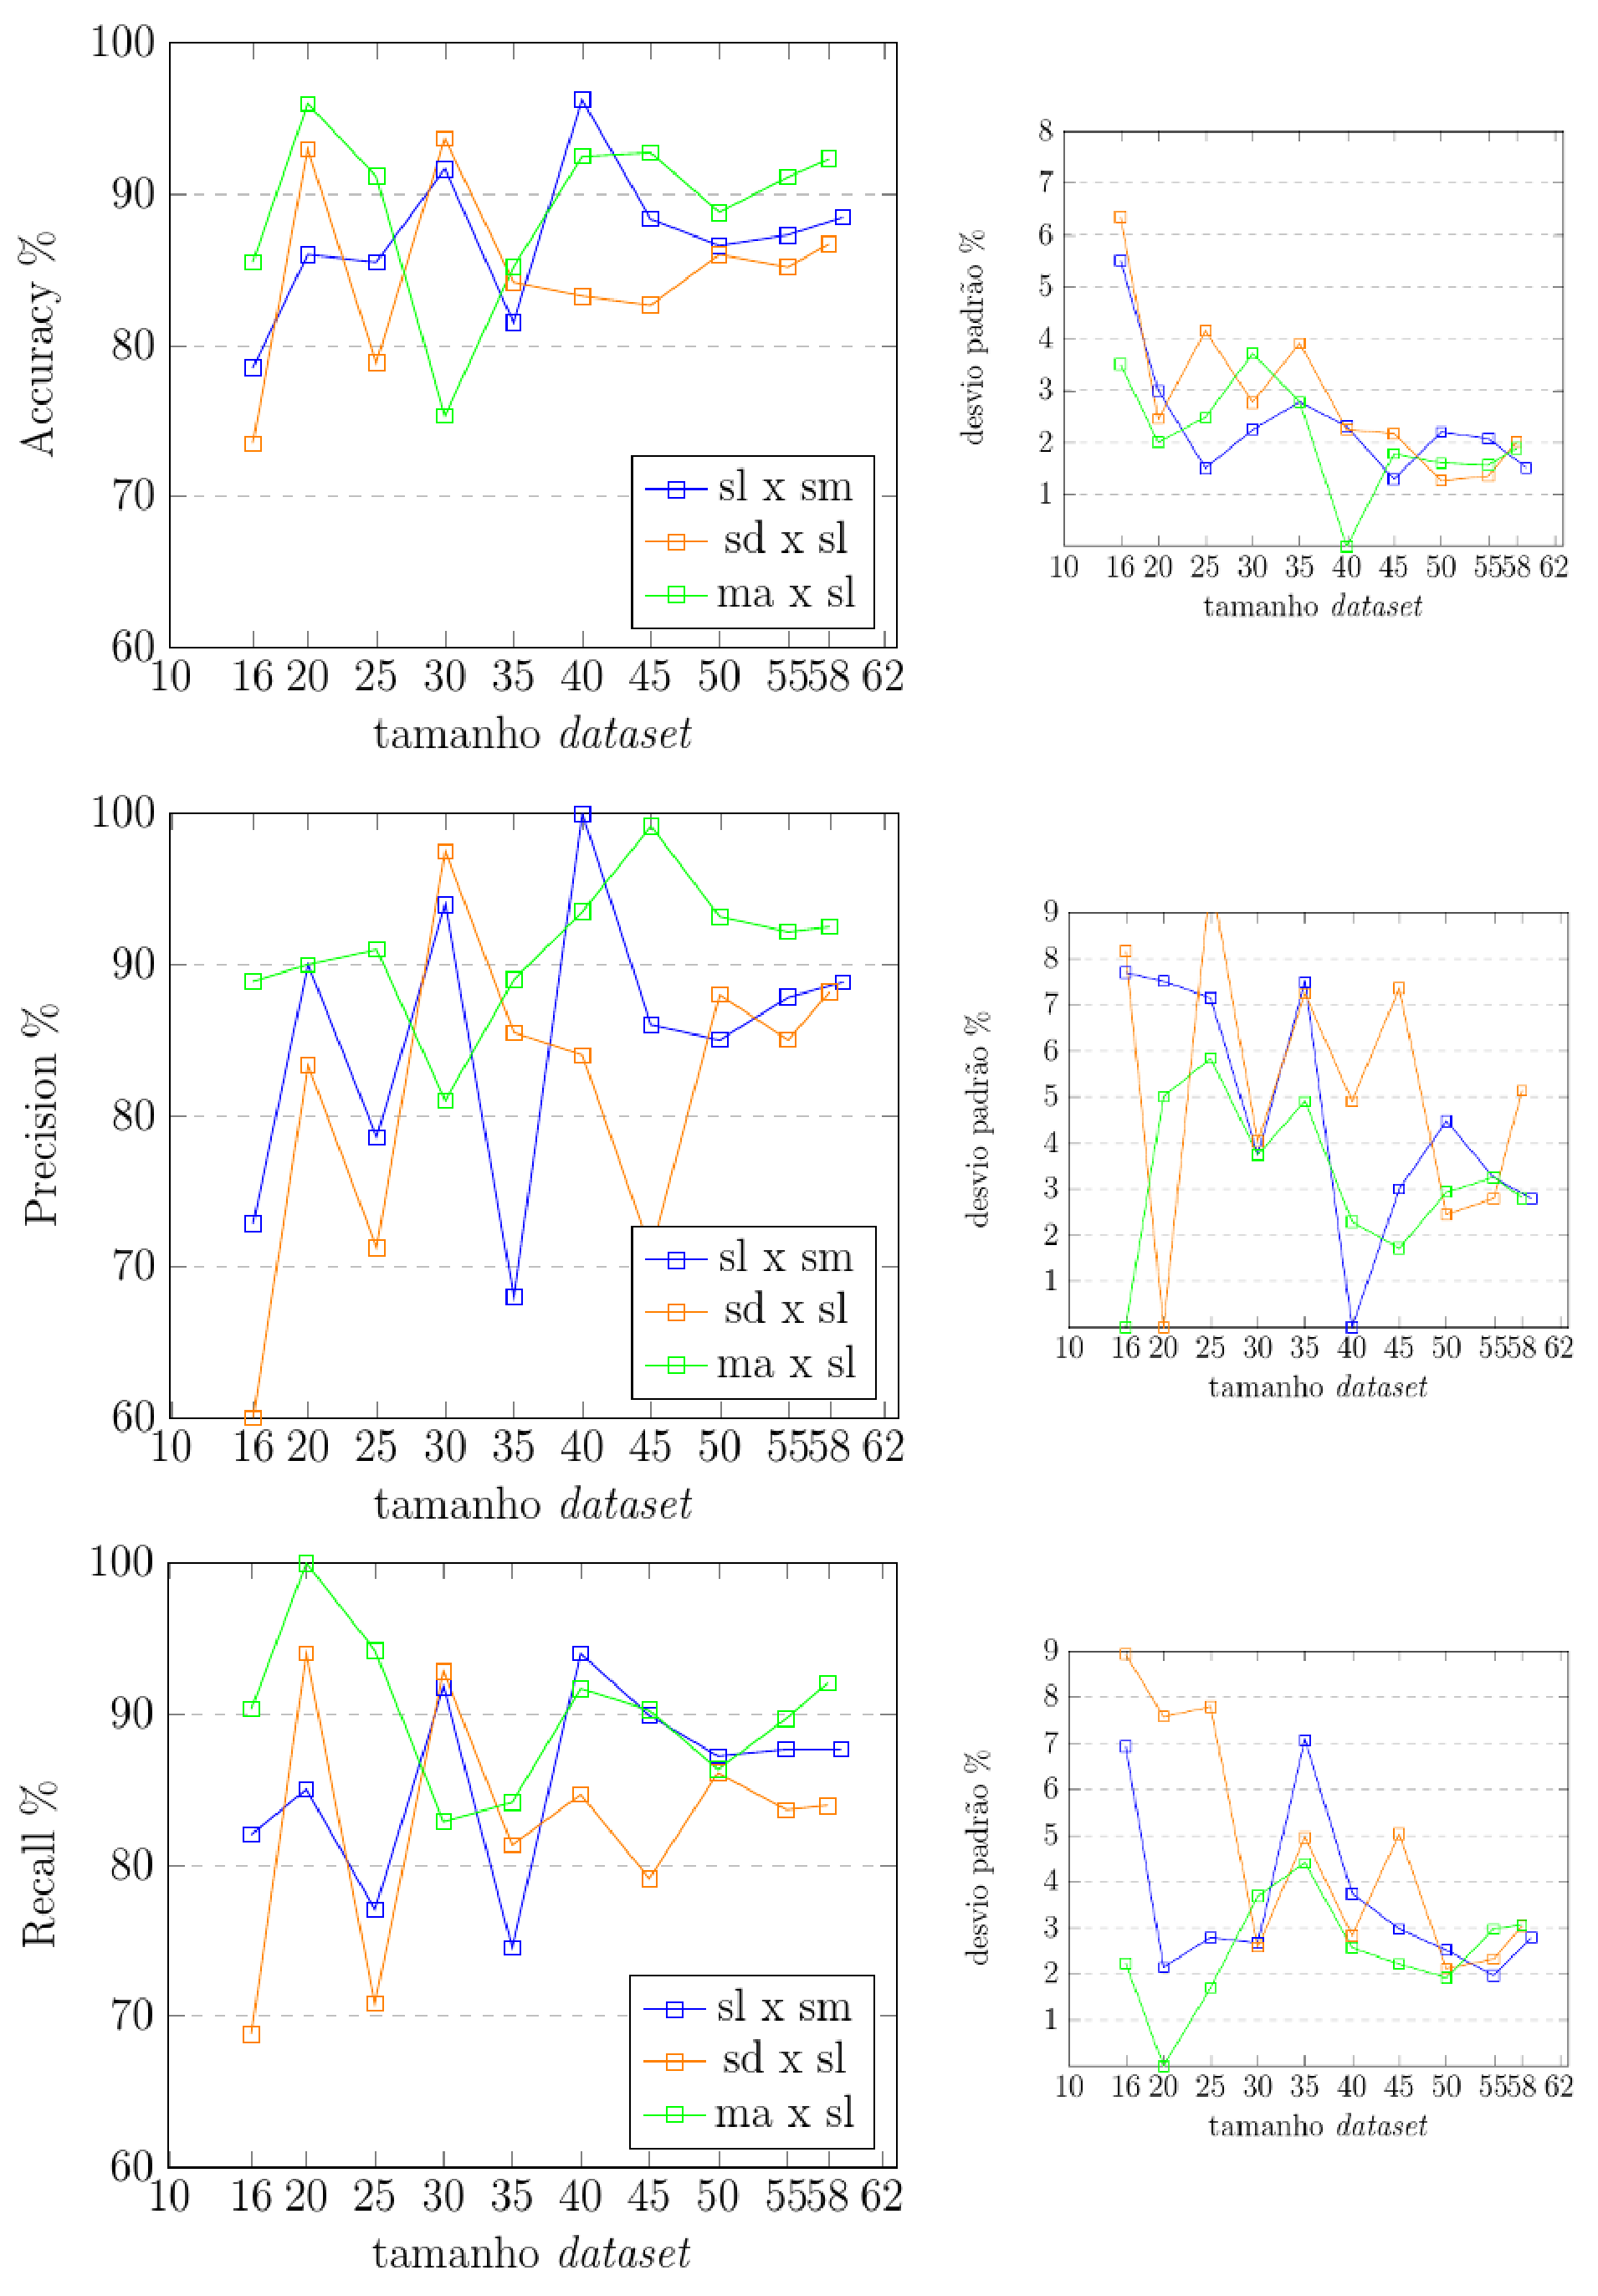
\includegraphics[width=1.0\columnwidth]{experimento/accuracy_precision_recall} 
  \caption{\textit{Accuracy}, \texit{Precision} e \textit{Recall} obtidas utilizando stratified-10-fold-crossvalidation (repetido 10 vezes) e DECORATE sobre diferentes frações do \textit{dataset} com os pares de parâmetros  selecionados na seção \ref{sec:selecaodados}.} 
  \label{fig:accuracy_precision_recall}
\end{figure}

\begin{table}[!htp]
  \centering
  \begin{tabular}{ |l|c c c c c|}
    \hline
       {\bf \textbf{$n^o i$}} & {\bf 40} & {\bf 45} & {\bf 50} & {\bf 55} & {\bf 58} \\
    \hline
       \textbf{A, DP} & 92.5, 0 & 92.75, 1.78 & 88.8, 1.6 & 91.13, 1.56 & 92.33, 1.89 \\
    \hline
       \textbf{P, DP} & 93.5, 2.29 & 99.17, 1.71 & 93.17, 2.93 &  92.17, 3.25 & 92.5, 2.81 \\
    \hline
       \textbf{R, DP} & 91.69, 2.56 & 90.25, 2.21 & 86.33, 1.91 & 89.71, 2.97 & 92.05, 3.06 \\
    \hline
  \end{tabular}
  \caption{Valores das curvas ``ma x sl'' da Figura \ref{fig:accuracy_precision_recall} a partir do \textit{dataset} com 40 instâncias. A (\textit{Accuracy}), P (\textit{Precision}, R (\textit{Recall}), DP (Desvio Padrão), i (instâncias). Os valores A, P, R e DV estão em \%.}
  \label{table:valorescurva}
\end{table}

Finalizando a análise decidiu-se que o melhor ponto para poder se construir um classificador é o com $n^o i = 45$, pois além de se ter um alto grau de \textit{recall} e \textit{accuracy} têm-se também \textit{precision} quase de 100\%. Então, para se construir um classificador final com base neste modelo escolheu-se randomicamente 45 instâncias do \textit{dataset} de 59 instâncias e aplicou-se \textit{stratified-10-fold-cross-validation} (repetido dez vezes). Este procedimento foi repetido diversas vezes (Figura \ref{fig:apr45_dev}) até que se obtivesse um modelo que satisfizesse a expressão \ref{eq:esxpvalclass}. O modelo que satisfez essa expressão obteve resultados que podem ser vistos na Tabela \ref{table:valmodelfinal} e este será o modelo final de classificador que será implantado no FIM. 

\begin{equation}
  (\textit{accuracy} \geq (92.75-1.78)) \wedge (\textit{precision} \geq (99.17-1.71)) \wedge (\textit{recall} \geq 90.25)
  \label{eq:esxpvalclass}
\end{equation}

\begin{table}[!htp]
  \centering
  \begin{tabular}{ |l|c|c|}
    \hline
       {\bf } & {\bf } & {\bf DP \%} \\
    \hline
       \textbf{Accuracy} \% & 98.05 & 1.81 \\
    \hline
       \textbf{Precision} \% & 98.5 & 3.2 \\
    \hline
       \textbf{\textit{Recall} \%} & 97.67 & 2 \\
    \hline
  \end{tabular}
  \caption{Valores da validação do modelo final. DP (Desvio Padrão).}
  \label{table:valmodelfinal}
\end{table}

\begin{figure}[!htb] \centering 
  \centering
  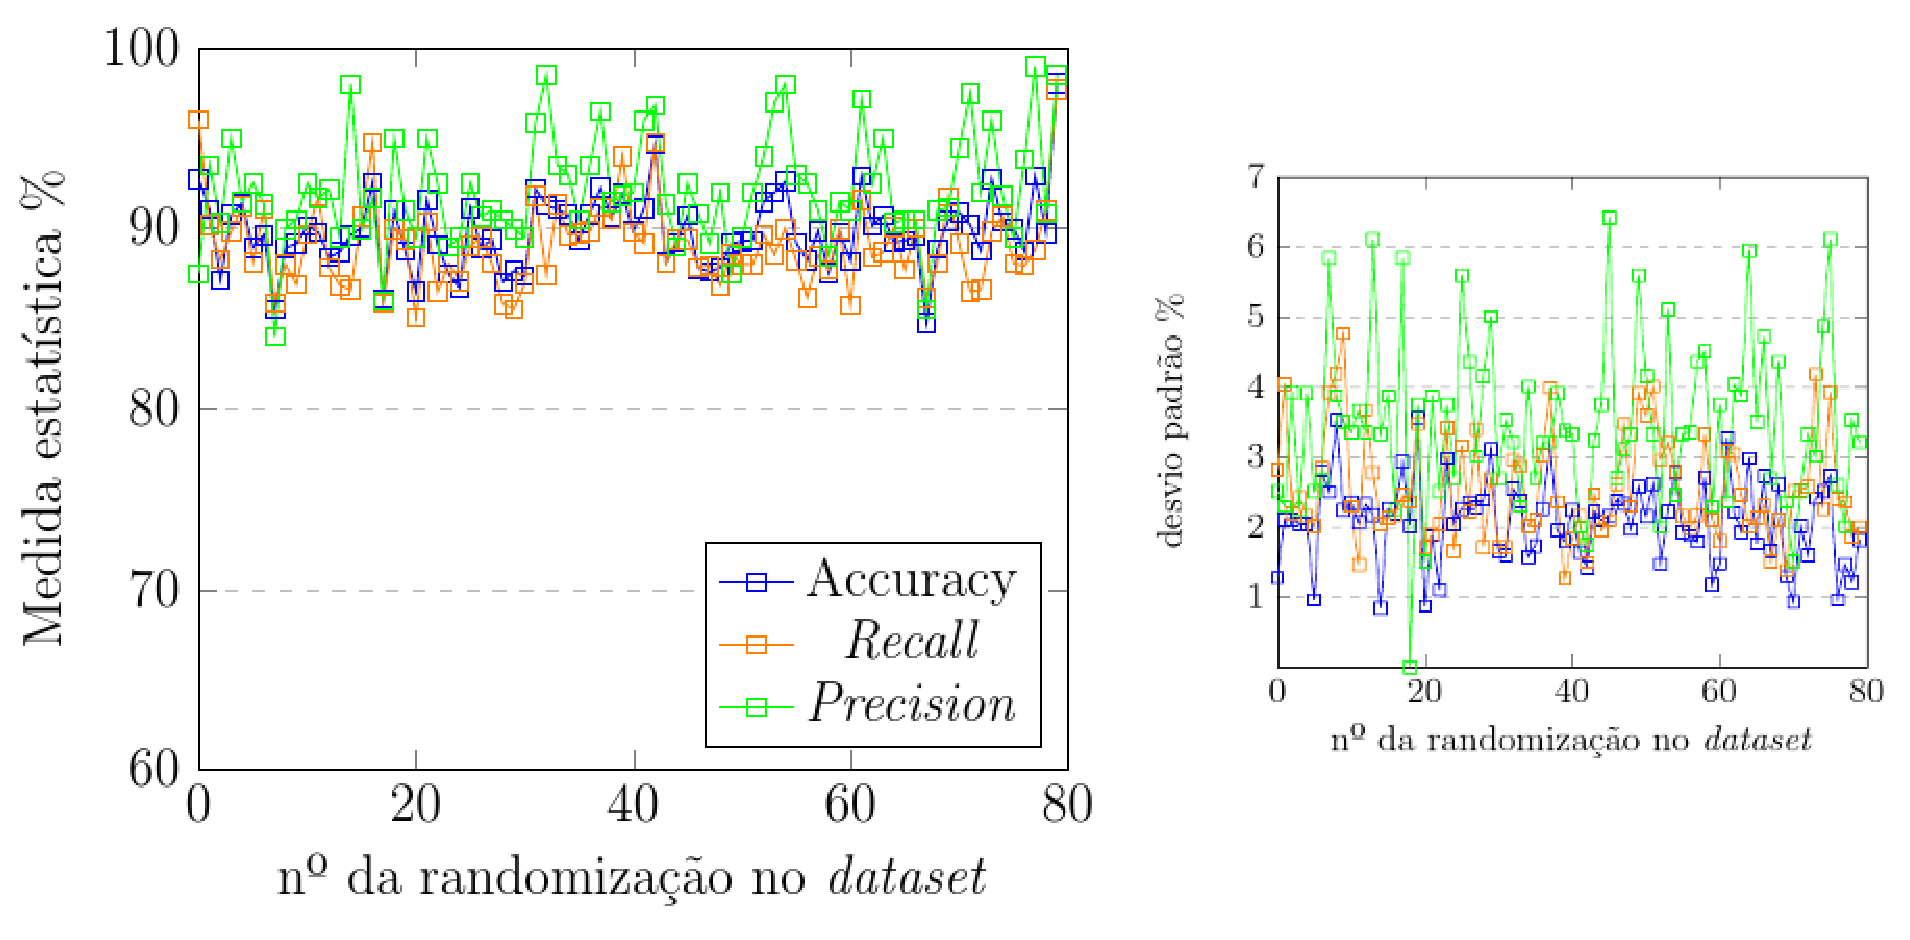
\includegraphics[width=1.0\columnwidth]{experimento/apr45_dev} 
  \caption{\textit{stratified-10-fold-cross-validation} (repetido dez vezes). 45 instâncias foram escolhidas randomicamente em cima do \textit{dataset} de 59 instâncias. Procedimento repetido até que satisfizesse a expressão \ref{eq:esxpvalclass} } 
  \label{fig:apr45_dev}
\end{figure}

\section{Resultados}
\label{sec:resultados}
Como provado na seção \ref{sec:constvalidacao} é possível construir um modelo de classificador que tenha um alto grau de generalização para o problema observado na seção \ref{subsec:obsproblema}. Sendo assim este foi implantado no FIM do HNS (Figura \ref{fig:hnsworkmodel}) afim de detectar efeitos colaterais indesejáveis no cenário da Figura \ref{fig:cenario}.

O classificador atua exatamente no momento em que o serviço veículo responde a requisição do FIM na etapa 3 da Figura (\ref{fig:cenario}). Nesta etapa o veículo primeiramente captura o ``id\_cesta'' (banco de dados) passado a ele pelo FIM. Então o veículo utiliza uma funcionalidade do serviço FIM que captura a cesta correspondente ao ``id\_cesta'', transforma-a em um arquivo ``arff'' contendo somente uma instância com os parâmetros correspondentes a ``somaLargura, mediaAltura, classe'', sendo a classe com valor não rotulado (valor esquecido), ou seja, não sabe-se a qual classe pertence (``é efeito colateral'' ou ``não é efeito colateral''). O FIM então salva este arquivo e retorna o caminho do arquivo como resposta para o dispositivo veículo. O veículo então responde a requisição 3, sendo um dos dados o caminho do arquivo ``arff'' referente a cesta. Neste momento o FIM utiliza o classificador (uma funcionalidade interna) para predizer se ``é efeito colateral'' ou ``não é efeito colateral'' passando como parâmetro ao classificador o caminho do arquivo ``arff''. Caso o classificador classifique como ``é efeito colateral'' o FIM interrompe o serviço e manda uma mensagem para o usuário. Caso contrário o fluxo do cenário (Figura \ref{fig:cenario}) continua.
